% !TeX root = ../main.tex

\section{Crystal lattice}

\begin{problem}[Crystallographic restriction theorem]
  Proof the crystallographic restriction theorem: Consider a crystal (i.e. with
  translational symmetry) in three dimensions that is invariant under rotations
  by an angle $2\pi/n$ around an axis. Then the only allowed possibilities are
  $n = 1$, $2$, $3$, $4$, $6$ with the case $n = 1$ being the trivial case
  with no rotational symmetry.
\end{problem}
\begin{solution}\begin{proof}
  Denote the 3D lattice can be generated by the basis vectors
  $\bm e_1$, $\bm e_2$, and $\bm e_3$.
  So, any lattice point vector set should be
  \[
    \bm L = \{a_1 \bm e_1 + a_2 \bm e_2 + a_3 \bm e_3\}.
  \]
  Obviously, $a_i \in \mathbb Z$, i.e., any lattice point can be labeled
  by integer coordinates $(a_1, a_2, a_3)$.
  Consider the 3D rotation matrix (operator)
  \[
    \mathbf R = \begin{pmatrix}
      \cos\theta & -\sin\theta & 0\\
      \sin\theta & \cos\theta & 0\\
      0 & 0 & 1
    \end{pmatrix}.
  \]
  When acting it on the vector $\bm L$, it should leave the lattice invariant,
  i.e., the trace must be integers
  \[
    \Tr(\mathbf R) = 2\cos\theta + 1 \in \mathbb Z.
  \]
  So we have $2\cos\theta = 2\cos(2\pi/n) \in \mathbb Z$, i.e.,
  $\cos(2\pi/n) = -1$, $-1/2$, $0$, $1/2$, $1$, then $n \in \{1,2,3,4,6\}$.
\end{proof}
\end{solution}

\begin{paracol}{2}
\begin{problem}[2D triangular lattice]
  Let us consider a two-dimen\-sional triangular lattice as shown in following
  Figure.
  \begin{enumext}
    \item Identify the primitive unit cell of the two-dimensional triangular
    lattice. Find the basis vectors.
    \item Construct the basis vectors of the reciprocal unit cell.
  \end{enumext}
\end{problem}
\switchcolumn \vspace*\fill
\centering
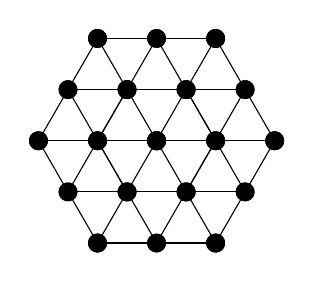
\begin{tikzpicture}[scale = .75]
  \foreach \i in {0, 1, 2, 3, 4, 5} {
    \foreach \j in {0, 1, 2} {
      \draw [rotate around = {-\i * 60:(0,0)}]
        ({-2 + \j/2}, {sqrt(3)*\j/2}) --++ (2,0);
        \foreach \k in {0, 1, 2}
          \fill [rotate around = {-\i * 60:(0,0)}]
            ({-\j + \k/2}, {sqrt(3)*\k/2}) circle (.16);
    }
    \draw [rotate around = {-\i * 60:(0,0)}] (-1,0) --++ (1,{sqrt(3)});
  }
\end{tikzpicture}
\vspace*\fill
\end{paracol}
\begin{solution}\leavevmode
  \begin{enumext}
    \item Denote the lattice constant $a$. Then the simplest choice of
    primitive lattice vectors is
    \[
      \bm a_1 = a    (1,0), \quad
      \bm a_2 = a \ab(\frac12, \frac{\sqrt3}{2}).
    \]
    \item Denote the two reciprocal-lattice primitive vectors
    $\bm b_1 = (b_{1_x}, b_{1_y})$, $\bm b_2 = (b_{2_x}, b_{1_2})$.
    Using the relation
    \[
      \bm a_i \cdot \bm b_j = 2\pi\delta_{ij}.
    \]
    To expand it
    \[
      \bm a_1 \cdot \bm b_1 = 2\pi, \quad
      \bm a_2 \cdot \bm b_1 = 0, \quad
      \bm a_1 \cdot \bm b_2 = 2\pi, \quad
      \bm a_2 \cdot \bm b_2 = 2\pi,
    \]
    we obtain the two reciprocal-lattice primitive vectors
    \[
      \bm b_1 = \frac{2\pi}a \ab(1, -\frac1{\sqrt3}), \quad
      \bm b_2 = \frac{2\pi}a \ab(0, \frac2{\sqrt3}).
    \]
  \end{enumext}
\end{solution}

\begin{problem}[Properties of the reciprocal lattice]\leavevmode
  \begin{enumext}
    \item Show that all reciprocal lattice vectors of the form
    $\bm G = h\bm A + k\bm B + l\bm C$ are perpendicular to the planes of the
    same indices $(h, k, l)$ in real space.
    \item Show that the distance $d_{h,k,l}$ between two consecutive planes
    $(h, k, l)$ is inversely proportional to $|\bm G_{h,k,l}|$.
    \item Find $d_{h,k,l}$ for a simple cubic lattice and an orthorhombic
    lattice ($a \neq b \neq c$, $\alpha = \beta = \gamma = \pi/2$).
  \end{enumext}
\end{problem}
\begin{solution}\leavevmode`'
  \begin{enumext}
    \item \begin{proof}
      Substitute the expressions of the reciprocal lattice vectors to $\bm G$
      \[
        \bm G = \frac{2\pi}{V}
           [h(\bm a_2 \times \bm a_3) + k(\bm a_3 \times \bm a_1)
          + l(\bm a_1 \times \bm a_2)].
      \]
      Since the Miller indices $(h, k, l)$ correspond to a plane that
      intercepts the crystal axies at $\bm a_1/h$, $\bm a_2/k$, $\bm a_3/l$,
      then, any vector lying in the $(h, k, l)$ plane can be written as a linear
      combination of two independent vectors in that plane, i.e.,
      \[
        \bm r_1 = \frac{\bm a_2}{k} - \frac{\bm a_1}{h}, \quad
        \bm r_2 = \frac{\bm a_3}{l} - \frac{\bm a_2}{k}.
      \]
      Then, the normal to this plane can be written as a cross product
      \[
        \hat{\bm n}_{hkl} = \bm r_1 \times \bm r_2
      = \frac{1}{kl} (\bm a_2 \times \bm a_3) +
        \frac{1}{hl} (\bm a_3 \times \bm a_1) +
        \frac{1}{hk} (\bm a_1 \times \bm a_2).
      \]
      which is parallel to $\bm G$, implies that $\bm G$ is perpendicular to the
      $(h, k, l)$ plane.
    \end{proof}
    \item \begin{proof}
    For the vector pointing to the $n + 1$ and $n$-th $(h, k, l)$ plane,
    it satisfies
    \[
      \bm G \cdot \bm r_{n+1} = 2\pi(n + 1), \qq{and}
      \bm G \cdot \bm r_n = 2\pi n,
    \]
    where $\bm r_{n+1} - \bm r_n = d \hat{\bm n}$. Combine the two relations
    \[
      \bm G \cdot(\bm r_{n+1} - \bm r_n) = \bm G \cdot \bm{\hat n} d = 2\pi d.
    \]
    So, we have
    \[
      d = \frac{2\pi}{\bm G \cdot \bm{\hat n}} = \frac{2\pi}{|\bm G_{h,k,l}|},
    \]
    i.e., the distance between two consecutive planes is inversely proportional
    to $|\bm G_{h,k,l}|$.
    \end{proof}
    \item For a simple cubic lattice
    \[
      \bm a = (a,0,0), \quad \bm b = (0,b,0), \quad \bm c = (0,0,c).
    \]
    Then, the reciprocal vectors can be expressed as
    \[
      \bm G = \frac{2\pi h}{a} \bm{\hat x} +
              \frac{2\pi k}{b} \bm{\hat y} +
              \frac{2\pi l}{c} \bm{\hat z},
    \]
    and its magnitude
    \[
      |\bm G| = 2\pi \sqrt{\frac{h^2}{a^2} + \frac{k^2}{b^2} + \frac{l^2}{c^2}}.
    \]
    So, we obtain the distance $d = \frac{2\pi}{|\bm G|}
    = \ab(\frac{h^2}{a^2} + \frac{k^2}{b^2} + \frac{l^2}{c^2})^{-1/2}$.
  \end{enumext}
\end{solution}

\begin{problem}[Atomic planes and Miller indices: application to lithium]
  The Bravais lattice of lithium is simple cubic with lattice parameter
  $a = \qty{3.48}\angstrom$.
  \begin{enumext}
    \item Suppose that the atoms (assumed to be spheres) are placed along the
    $[111]$, represent the atomic distribution along the following faces
    $(100)$, $(110)$, $(111)$, and $(201)$.
    \item For each such 2D structure, state the direction and basis vector,
    $\bm a$ and $\bm b$ of the elementary lattice as well as the value of the
    angle, $\gamma$.
    \item Find the atomic concentration and the mass density of lithium
    ($A \approx 7$).
  \end{enumext}
\end{problem}
\begin{solution}\leavevmode
  \begin{enumext}
    \item (b)\quad
    The distribution, basis vector, and the angle of the faces are listed.
    \begin{center}
      \begin{tabular}{*5l}
        \toprule
        2D Structure & Distribution & $\bm a$ & $\bm b$ & $\gamma$\\
        \midrule
        $(100)$ & square      & $(0, a, 0)$   & $(0, 0, a)$ &
        $\qty{90}\degree$\\
        $(110)$ & rectangular & $(a, -a, 0)$  & $(0, 0, a)$ &
        $\qty{90}\degree$\\
        $(111)$ & hexagonal   & $(a, 0, -a)$  & $(0, a, -a)$ &
        $\qty{60}\degree$\\
        $(201)$ & rectangular & $(0, a, 0)$   & $(a, 0, -2a)$ &
        $\qty{90}\degree$\\
        \bottomrule
      \end{tabular}
    \end{center}
    \addtocounter{enumXi}{1}
    \item Since the atoms are placed along the $[111]$, then every cubic
    lattice's corners has an atom, i.e., it is equivalent that there is an
    atom in every lattice. So, the atomic concentration is
    \[
      n = \frac1V = \frac1{a^3} = \qty{2.3728e28}{atoms/\m^3}.
    \]
    The mass density is
    \[
      \rho = n m_\text{atom} = \frac{nA}{N_A} = \qty{275.816}{\kg/\m^3}.
    \]
  \end{enumext}
\end{solution}